\documentclass{ximera}[font=12pt]


\title{Adding Integers: Commutative Property}   % Use xmlatex all -s to compile when SERVE refuses to work.
\author{Kelly Stady}
\license{CC: 0}         % replace with an appropriate license, or set it in xmPreamble

\begin{document}

\begin{abstract}

\end{abstract}

\maketitle
\label{xim:AddIntCommPropActivity}


\section*{The Commutative Property of Addition}

The operation of addition is \textbf{commutative}, meaning numbers can be added in any order without changing the result.  For example,

\[ 4 + 3 = 3 + 4. \]

When adding multiple numbers with different signs, we can use this property to work more efficiently. Instead of working from left to right, simply combine the positive numbers and the negative numbers separately, then add those results.

\bigskip

\begin{example}  \ Find the sum $-6 + 3 + (-4) + 1.$
\begin{center}
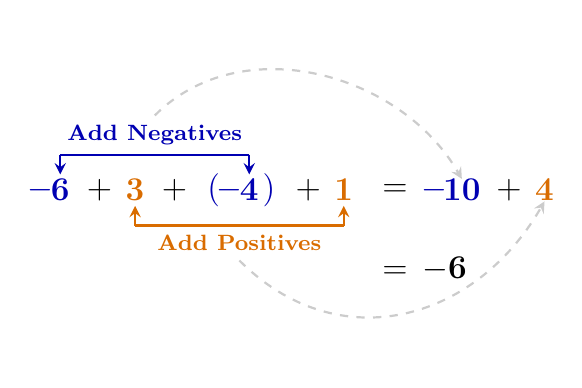
\begin{tikzpicture}[
    >=stealth,
    node distance=0.6cm,
    % Define Accessible Colors locally
    posColor/.style={color=orange!85!black},
    negColor/.style={color=blue!70!black}
]

    % --- LINE 1: THE FULL EXPRESSION ---
    % Negative 6
    \node[negColor, font=\large, inner sep=0pt] (n1minus) at (0,0) {$\mathbf{-}$};
    \node[negColor, font=\large, inner sep=0pt] (n1digit) at (0.25,0) {$\mathbf{6}$};

    \node[font=\large] (plus1) at (0.75,0) {$\mathbf{+}$};

    % Positive 3
    \node[posColor, font=\large, inner sep=0pt] (p1digit) at (1.2,0) {$\mathbf{3}$};

    \node[font=\large] (plus2) at (1.7,0) {$\mathbf{+}$};

    % Negative 4
    \node[negColor, font=\large, inner sep=0pt] (n2parenL) at (2.2,0) {$\mathbf{(}$};
    \node[negColor, font=\large, inner sep=0pt] (n2minus) at (2.4,0) {$\mathbf{-}$};
    \node[negColor, font=\large, inner sep=0pt] (n2digit) at (2.65,0) {$\mathbf{4}$};
    \node[negColor, font=\large, inner sep=0pt] (n2parenR) at (2.9,0) {$\mathbf{)}$};

    \node[font=\large] (plus3) at (3.4,0) {$\mathbf{+}$};

    % Positive 1
    \node[posColor, font=\large, inner sep=0pt] (p2digit) at (3.85,0) {$\mathbf{1}$};

    % --- RESULTS ON RIGHT (Identical thickness via \mathbf) ---
    \node[font=\large] (equals1) at (4.5,0) {$\mathbf{=}$};

    \node[negColor, font=\large, inner sep=0pt] (res1minus) at (5.0,0) {$\mathbf{-}$};
    \node[negColor, font=\large, inner sep=0pt] (res1digit) at (5.35,0) {$\mathbf{10}$};

    \node[font=\large] (plusFinal) at (5.95,0) {$\mathbf{+}$};

    \node[posColor, font=\large, inner sep=0pt] (res2digit) at (6.4,0) {$\mathbf{4}$};

    % --- TOP HORIZONTAL BAR (Negatives) ---
    \draw[negColor, thick] (0.25, 0.45) -- (2.65, 0.45);
    \draw[->, negColor, thick] (0.25, 0.45) -- (0.25, 0.2);
    \draw[->, negColor, thick] (2.65, 0.45) -- (2.65, 0.2);
    \node[negColor, font=\footnotesize\bfseries, anchor=south] (labelNeg) at (1.45, 0.45) {Add Negatives};

    % --- BOTTOM HORIZONTAL BAR (Positives) ---
    \draw[posColor, thick] (1.2, -0.45) -- (3.85, -0.45);
    \draw[->, posColor, thick] (1.2, -0.45) -- (1.2, -0.2);
    \draw[->, posColor, thick] (3.85, -0.45) -- (3.85, -0.2);
    \node[posColor, font=\footnotesize\bfseries, anchor=north] (labelPos) at (2.525, -0.45) {Add Positives};

    % --- FLOW INDICATORS ---
    \draw[->, gray!40, dashed, thick] (labelNeg.north) to [out=45, in=120] (res1digit.north);
    \draw[->, gray!40, dashed, thick] (labelPos.south) to [out=315, in=240, looseness=1.15] (res2digit.south); % lossness increases the sag

    % --- LINE 2: FINAL BOLD RESULT ---
    \node[font=\large, anchor=west] (final) at (equals1.west) [yshift=-1.0cm] {$\mathbf{= \, -6}$};

\end{tikzpicture}
\end{center}

\end{example}

\begin{problem}
Use the commutative property to find each sum.

\[ -5 + 2 + (-4) + 8 \begin{prompt} = \answer{1} \end{prompt} \]


\[ 3 + (-1) + 6 + (-15) + 1  \begin{prompt} = \answer{-6} \end{prompt} \]

\end{problem}

~ \\[2em]

% Newspaper - Extra Extra!

\begin{tikzpicture}[scale = 0.45]
    % Paper Base (approx 2cm x 2cm / 0.8in)
    \draw[thick, fill=white] (0,0) rectangle (2,2);

    % Headline (Bold line)
    \draw[ultra thick, black!80] (0.2, 1.7) -- (1.8, 1.7);

    % Secondary Headline (Thin line)
    \draw[very thin, black!60] (0.2, 1.5) -- (1.2, 1.5);

    % "Image" Box
    \draw[fill=gray!20] (0.2, 0.8) rectangle (0.9, 1.3);
    \draw[gray!50, ultra thin] (0.2, 0.8) -- (0.9, 1.3) (0.2, 1.3) -- (0.9, 0.8);

    % Text Lines (Column 1 - below image)
    \foreach \y in {0.6, 0.4, 0.2}
        \draw[ultra thin, black!40] (0.2, \y) -- (0.9, \y);

    % Text Lines (Column 2 - full height)
    \foreach \y in {1.3, 1.1, 0.9, 0.7, 0.5, 0.3}
        \draw[ultra thin, black!40] (1.1, \y) -- (1.8, \y);
\end{tikzpicture}


\subsection*{Great News!}

The rules for adding integers apply to all \textbf{real numbers}. The integers, along with the fractions and decimals between them, make up the set of
real numbers—more on that later.  Did you know that there are infinitely many numbers between each integer?

Once you have mastered these addition rules, you will be ready for subtraction. As you will see in the next lesson,
\textbf{if you can add integers, you can subtract them too!}


\end{document}